\documentclass[12pt]{article}
\usepackage[english]{babel}
\usepackage[utf8]{inputenc} % Permite el uso de caracteres del Español
\usepackage[T1]{fontenc}
\usepackage{graphicx}
\usepackage{amsmath}
\usepackage{wrapfig}
\usepackage{enumerate}
\usepackage[top=1in, bottom=1.25in, left=1.1in, right=1.1in]{geometry}
\usepackage[dvipsnames]{xcolor}
\usepackage{subcaption}

\begin{document}

\begin{titlepage}

\newcommand{\HRule}{\rule{\linewidth}{0.5mm}} % Define un comando para las lineas horizontales

\center 
%----------------------------------------------------------------------------------------
%	Cabezera
%----------------------------------------------------------------------------------------

\textsc{\LARGE Universidad de Sonora}\\[1.5cm]
\textsc{\Large Licenciatura en Física}\\[0.5cm]
\textsc{\large Física Computacional I}\\[0.5cm]

%----------------------------------------------------------------------------------------
%	Titulo
%----------------------------------------------------------------------------------------

\HRule \\[0.4cm]
{\huge \bfseries Actividad 7 - Sistema de resortes acoplados Completo}\\[0.4cm] % Title of your document
\HRule \\[1.5cm]
 
%----------------------------------------------------------------------------------------
%	Autor
%----------------------------------------------------------------------------------------

\begin{minipage}{0.4\textwidth}
\begin{flushleft} \large
\emph{Alumno:}\\
José Gabriel Navarro I.
\end{flushleft}
\end{minipage}
~
\begin{minipage}{0.4\textwidth}
\begin{flushright} \large
\emph{Profesor:} \\
Carlos Lizarraga Celaya
\end{flushright}
\end{minipage}\\[2cm]


%----------------------------------------------------------------------------------------
%	Fecha
%----------------------------------------------------------------------------------------
23 de Marzo de 2018

%----------------------------------------------------------------------------------------
%	Escudo
%----------------------------------------------------------------------------------------


\includegraphics[width=0.4\textwidth]{logo.png}\\
 
%----------------------------------------------------------------------------------------

\vfill % Llena el espacio de la pagina en blanco

\end{titlepage}

\section{Introducción}
En el presente reporte se complementa la sexta actividad realizada para la clase de Física Computacional I, en donde ademas abarcar el análisis de las ecuaciones de un sistema de resortes acoplados, se habla tambien acerca de los sistemas no lineales y forzados. \\

Se presenta la síntesis realizada la practica anterior, continuando con la nueva información acerca de sistemas no lineales y forzados del mismo articulo de Fay \& Graham, mostrando sus ecuaciones y código para resolver estos problemas numéricamente.  Al final se presenta una conclusión de la actividad, así como la bibliografía utilizada para la investigación de los fundamentos y el apéndice. 

\section{Síntesis - Sistema de resortes acoplados}

\subsection{Introducción}

\begin{wrapfigure}{r}{0.2\textwidth}
    \centering
    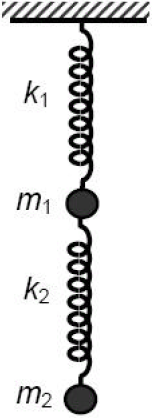
\includegraphics[width=0.1\textwidth]{ResorteAcoplado.png}
\end{wrapfigure}

En este artículo, se investiga uno de los problemas más interesantes de Mecánica, y que ahora normalmente se utiliza para la introducción al estudio de ecuaciones diferenciales. Este problema es el de dos resortes con dos masas puestas en serie, colgando del techo. Si suponemos que las fuerzas restauradoras de los resortes se comportan según la Ley de Hooke, estos dos grados de libertad nos dan un modelo de ecuaciones diferenciales lineales de segundo grado. Al sustituir una ecuación en la otra, el movimiento de las masas puede ser descrito por una ecuación diferencial lineal de cuarto grado.\\

Con estas ecuaciones, podemos investigar los movimientos de las dos masas, para saber si estas están sincronizadas (es decir en fase), o si son opuestas (en desfase). Además, también se puede observar gráficamente la periodicidad, la amplitud, la fase, y otros conceptos al modificar los parámetros de este modelo. 

\subsection{El modelo de los resortes acoplados}
Como se menciono anteriormente, el modelo consiste de dos resortes y dos masas. Un resorte, con una constante $k_1$, esta colgado del techo con una masa $m_1$ colgando de ella. De aquí, cuelga otro resorte con una constante de $k_2$ y debajo de ella cuelga una masa $m_2$.  Al dejarlo en reposo, los resortes se estiran una distancia, a la que llamaremos: $x_1$ y $x_2$. \\

\subsubsection{Asumiendo la Ley de Hooke}
Si asumimos que el sistema se mueve con oscilaciones pequeñas, podemos asumir que los resortes tendrán una fuerza restauradora dada por la Ley de Hooke, dada de la forma: $-k_1l_1$ y $-k_2l_2$ en donde $l_1$ y $l_2$ son las elongaciones o comprensiones de los dos resortes. Como $m_1$ esta atada a los dos resortes, en esta actuan las dos fuerzas restauradoras, mientras que $m_2$ solamente "siente" la fuerza restauradora del segundo resorte. Sin fricción, la segunda ley de Newton para estas dos masas son de la siguiente forma: \\

\centerline{$m_1 \ddot x_1 = -k_1x_1 - k_2(x_1-x_2)$}
\centerline{$m_2 \ddot x_2 = -k_2(x_2-x_1)$}
$    $

Para encontrar una ecuación para $x_1$ que no involucre a $x_2$, resolvermos la ecuación de $x_2$, y sustituyendo esta ecuación en las ecuaciones anteriores llegamos a la siguiente ecuación diferencial de cuarto grado: \\

\centerline{$m_1m_2x_1^{(4)} + (m_2k_1 + k_2(m_1+m_2)) \ddot x_1 + k_1k_2x_1=0$}
$    $

Y si se hace ese mismo proceso pero para $x_2$, se llega a la misma ecuación anterior. Solamente las posiciones y velocidades iniciales se necesitan para poder determinar la solución. 

\subsubsection{Algunos ejemplos con masas idénticas}
\noindent \textit{2.1 Describe el movimiento para un sistema de resortes con $k_1=6$ y $k_2=4$ con condiciones iniciales de $(x_1(0), \dot x_1(0), x_2(0), \dot x_2(0)$)=$(1,0,2,0)$.}\\

Resolviendo el problema de una forma analítica, podemos llegar a que las ecuaciones para las posiciones de las masas son: \\

\centerline{$x_1(t) = cos \sqrt 2 t$}
\centerline{$x_2(t) = 2 cos \sqrt 2 t$}
$ $

El movimiento esta sincronizado, y por lo tanto las masas se mueven en fase una con la otra. Solamente tienen amplitud diferentes. El retrato de fase de estas son elipses, y como solamente varían en amplitud, al graficar sus posiciones una contra otra, se obtiene una linea recta. A continuación se presenta el código utilizado para encontrar numéricamente estos resultados y las graficas correspondientes: \\ 

Para graficar los datos, solamente se utilizo la linea de código de lectura de datos: \textit{t, x1, xy, x2, y2, er1, er2 = loadtxt('dosresortes2\_1.dat', unpack=True)}, y se graficaron los datos como ya se ha echo anteriormente en otras practicas. \\ \\  

\begin{figure}[h!]
    \centering
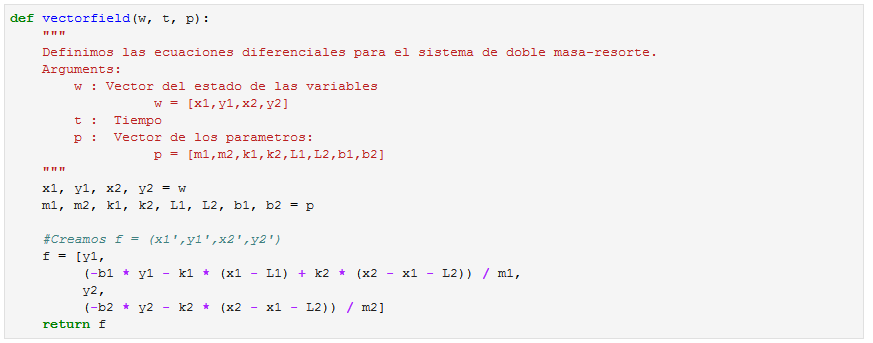
\includegraphics[width=6in]{Cod1.png}
\end{figure}

\begin{figure}[h!]
    \centering
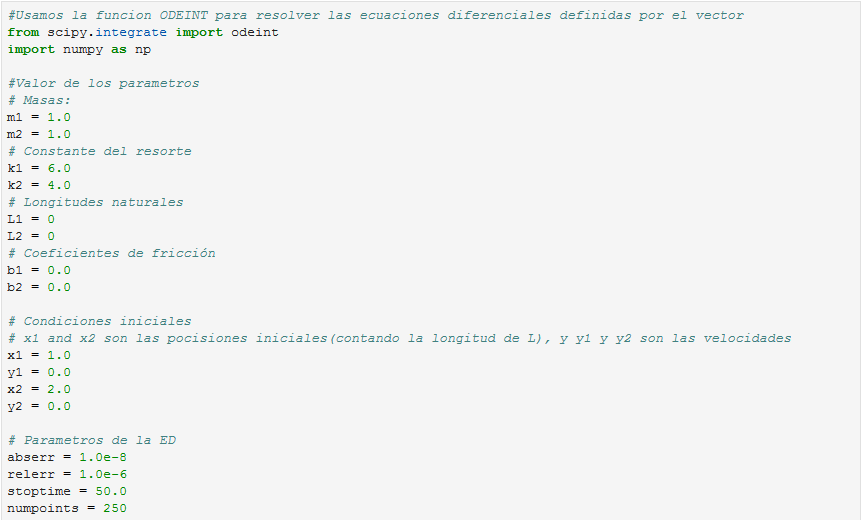
\includegraphics[width=6in]{Cod2.png}
\end{figure}

\begin{figure}[h!]
    \centering
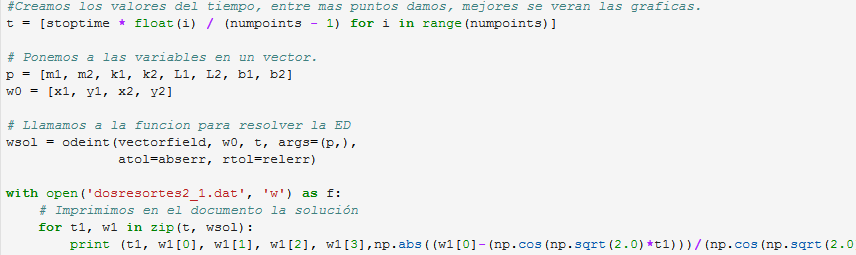
\includegraphics[width=6in]{Cod3.png}
\end{figure}

\clearpage

\begin{figure}[h!]
    \centering
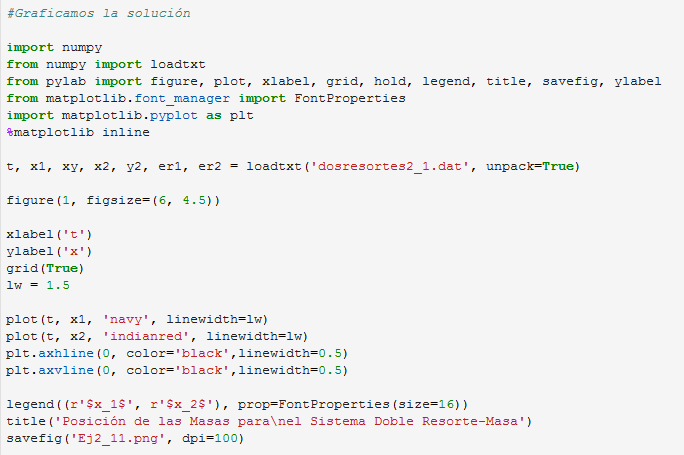
\includegraphics[width=6in]{Cod4.png}
\end{figure}

Las gráficas obtenidas son:
\begin{figure}[h!]
    \centering
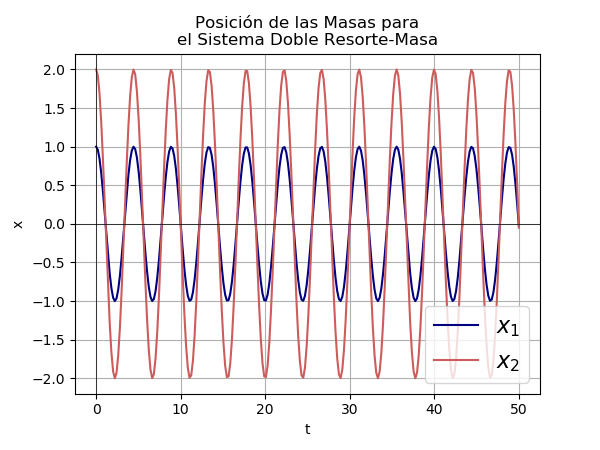
\includegraphics[width=5in]{Ej2_11.png}
\caption{Graficas de $x_1$ y $x_2$}
\end{figure}
\begin{figure}[h!]
\begin{subfigure}{.55\textwidth}
  \centering
  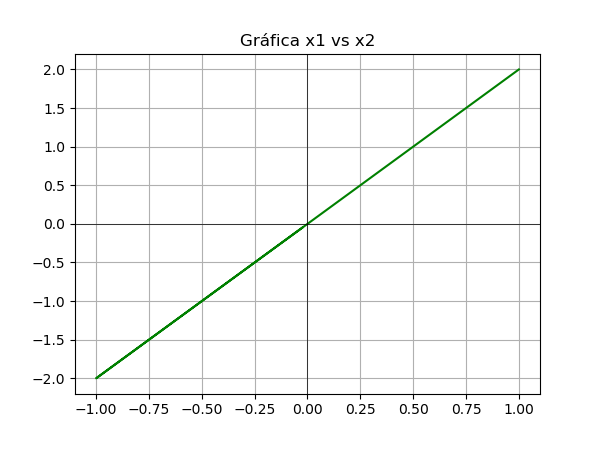
\includegraphics[width=.8\linewidth]{Ej2_12.png}
  \caption{$x_1$ vs $x_2$}
  \label{fig:sfig2}
\end{subfigure}
\begin{subfigure}{.55\textwidth}
  \centering
  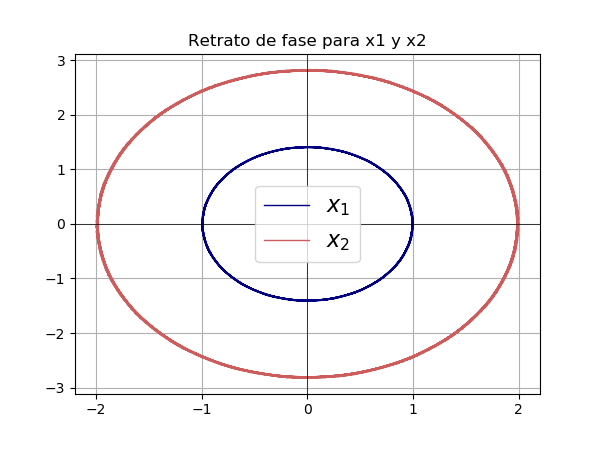
\includegraphics[width=.8\linewidth]{Ej2_13.png}
  \caption{Retrato de fase de $x_1$ y $x_2$}
  \label{fig:sfig2}
\end{subfigure}
\end{figure}

\noindent \textit{2.2 Describe el movimiento para un sistema de resortes con $k_1=6$ y $k_2=4$ con condiciones iniciales de $(x_1(0), \dot x_1(0), x_2(0), \dot x_2(0)$)=$(-2,0,1,0)$.}\\

Para este caso, la primera masa se mueve hacia abajo mientras que la otra se mueve hacia arriba, tienen el mismo periodo, pero estan fuera de fase. La solución analítica es: \\

\centerline{$x_1(t) = -2 cos 2\sqrt 3 t$}
\centerline{$x_2(t) = cos 2\sqrt 3 t$}
$ $

El código utilizado para este caso, es el mismo que se uso en el ejemplo anterior, y así fue con todos los ejemplos. Lo único que cambiaba eran los datos a utilizar y las graficas resultantes: 

\begin{figure}[h!]
    \centering
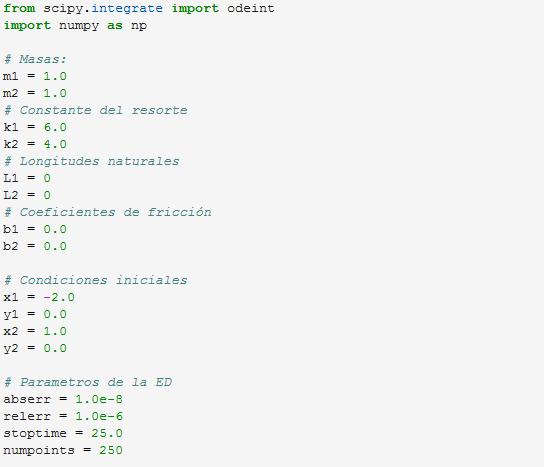
\includegraphics[width=3.5in]{Cod5.png}
\end{figure}

Las gráficas son:

\begin{figure}[h!]
\begin{subfigure}{.6\textwidth}
  \centering
  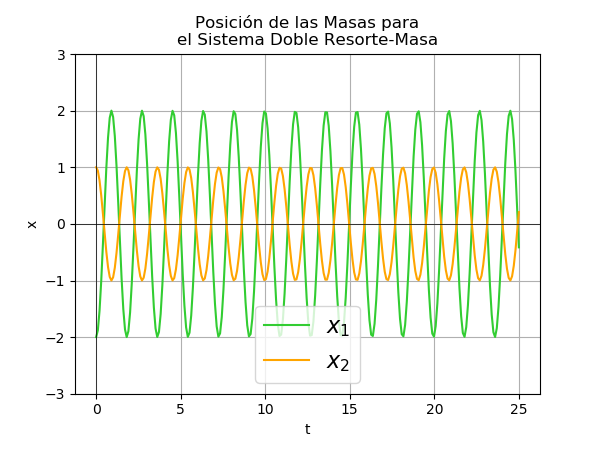
\includegraphics[width=.8\linewidth]{Ej2_21.png}
  \caption{Gráfica de $x_1$ y $x_2$}
  \label{fig:sfig2}
\end{subfigure}
\begin{subfigure}{.6\textwidth}
  \centering
  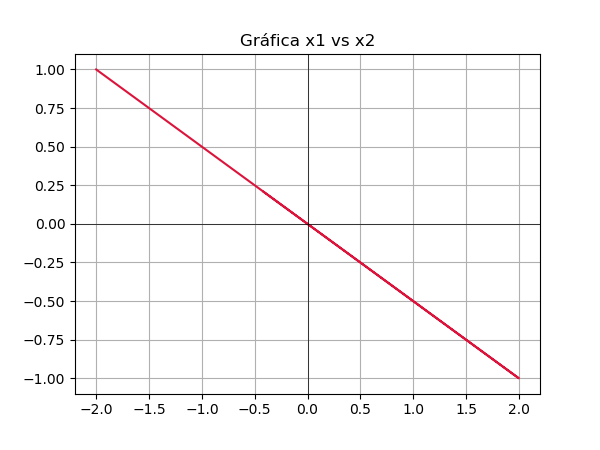
\includegraphics[width=.8\linewidth]{Ej2_22.png}
  \caption{Gráfica de $x_1$ vs $x_2$}
  \label{fig:sfig2}
\end{subfigure}
\end{figure}

\noindent \textit{2.3 Describe el movimiento para un sistema de resortes con $k_1=0.4$ y $k_2=1.808$ con condiciones iniciales de $(x_1(0), \dot x_1(0), x_2(0), \dot x_2(0)$)=$(1/2,0,-1/2,7/10)$.}\\

Con este ejemplo podemos observar como las condiciones iniciales solo afectan a la amplitud y fase de la soluciones, mientras que las constantes de los resortes determinan el periodo y frecuencia del fenómeno. Los retratos de fase son casi un movimiento periódico entre ellos, y si graficamos $x_1$ vs $x_2$ parece una curva de tipo Lissajous. En el código solamente se edito los datos como las constantes y las condiciones iniciales:

\begin{figure}[h!]
    \centering
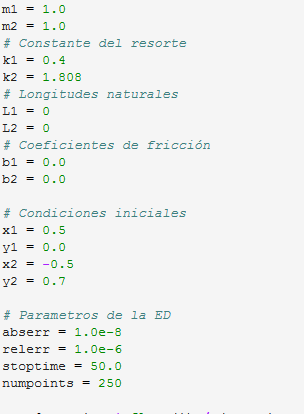
\includegraphics[width=3in]{Cod6.png}
\end{figure}

Las graficas resultantes fueron: \\ \\

\begin{figure}[h!]
\begin{subfigure}{.55\textwidth}
  \centering
  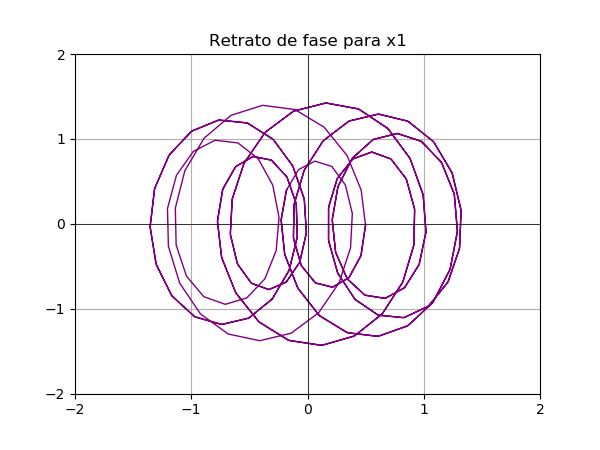
\includegraphics[width=.8\linewidth]{Ej2_31.png}
  \caption{Retrato de fase de $x_1$}
  \label{fig:sfig2}
\end{subfigure}
\begin{subfigure}{.55\textwidth}
  \centering
  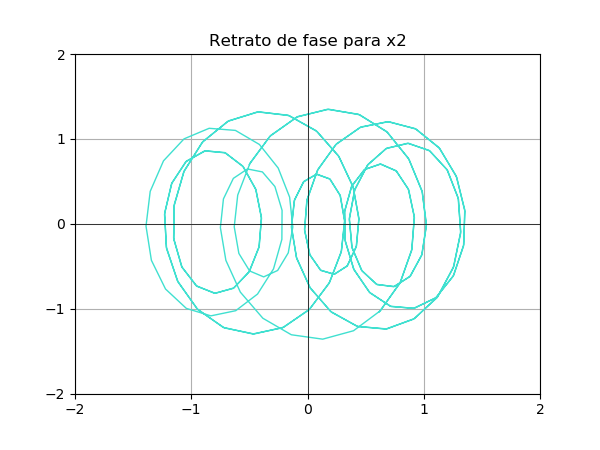
\includegraphics[width=.8\linewidth]{Ej2_32.png}
  \caption{Retrato de fase de $x_2$}
  \label{fig:sfig2}
\end{subfigure}
\begin{subfigure}{.55\textwidth}
  \centering
  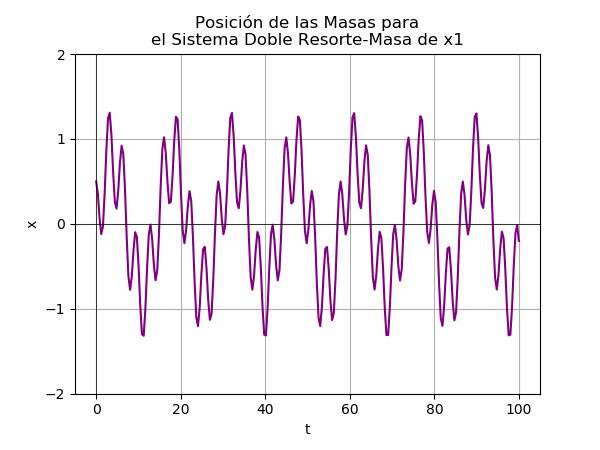
\includegraphics[width=.8\linewidth]{Ej2_33.png}
  \caption{Posición $x_1$ contra tiempo}
  \label{fig:sfig2}
\end{subfigure}
\begin{subfigure}{.55\textwidth}
  \centering
  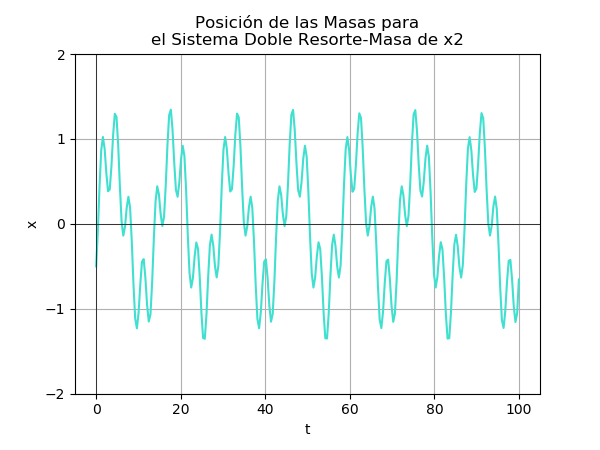
\includegraphics[width=.8\linewidth]{Ej2_34.png}
  \caption{Posición $x_2$ contra tiempo}
  \label{fig:sfig2}
\end{subfigure}
\begin{subfigure}{.55\textwidth}
  \centering
  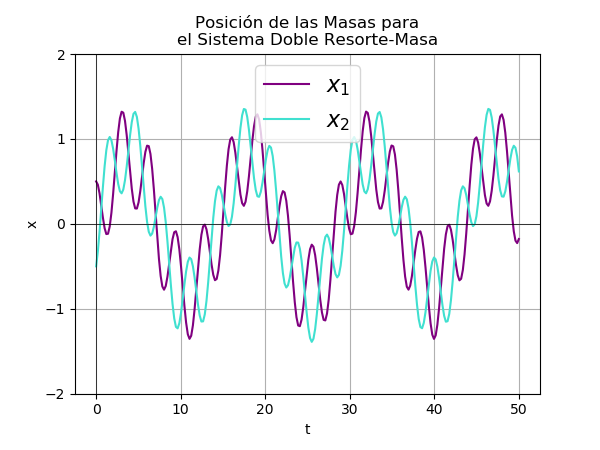
\includegraphics[width=.8\linewidth]{Ej2_35.png}
  \caption{Gráfica de $x_1$ y $x_2$}
  \label{fig:sfig2}
\end{subfigure}
\begin{subfigure}{.55\textwidth}
  \centering
  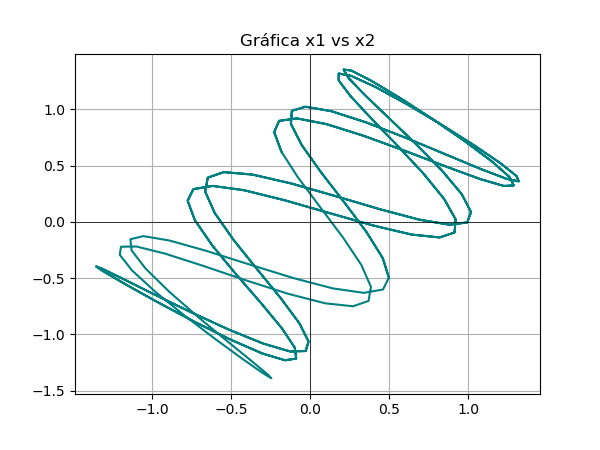
\includegraphics[width=.8\linewidth]{Ej2_36.png}
  \caption{Gráfica $x_1$ vs $x_2$}
  \label{fig:sfig2}
\end{subfigure}
\end{figure}

\subsection{Amortiguamiento}
Los problemas mas generales acerca de amortiguamiento es el de viscosidad, en donde la fuerza de amortiguamiento es proporcional a la velocidad. El amortiguamiento de la primera masa depende solamente de su velocidad y no en la de la segunda y viceversa. Si añadimos esta fuerza al modelo anteriormente descrito podemos obtener lo siguiente: \\

\centerline{$m_1 \ddot x_1 = -\delta \dot x_1 -k_1x_1 - k_2(x_1-x_2)$}
\centerline{$m_2 \ddot x_2 = -\delta \dot x_2 -k_2(x_2-x_1)$}
$    $

Se realiza el mismo proceso de obtener la ecuación de movimiento para una de las variables de posición, ya sea $x_1$ o $x_2$. Sustituimos esta ecuación en la anterior que le corresponde, y obtenemos de nuevo una ecuación diferencial lineal de cuarto grado para ambas posiciones de x. \\

\noindent \textit{2.4 Asume $m_1 = m_2 = 1$. Describe el movimiento para un sistema de resortes con $k_1=0.4$ y $k_2=1.808$, con coeficientes de amortiguamiento $\delta_1=0.1$ y $\delta_2=0.2$ con condiciones iniciales de $(x_1(0), \dot x_1(0), x_2(0), \dot x_2(0)$)=$(1,1/2,2,1/2)$.}\\

Como existe ahora un amortiguamiento, las amplitudes de ambos movimientos disminuyen conforme pasa el tiempo. Al graficar $x_1$ y $x_2$, podemos observar como se mueven casi en sincronía a pesar de que tienen distintas condiciones iniciales. El código para este caso es:  \\ 

\begin{figure}[h!]
    \centering
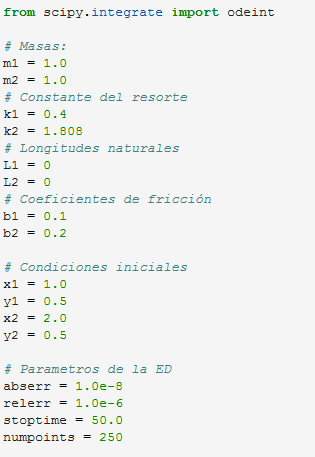
\includegraphics[width=2.5in]{Cod7.png}
\end{figure}

Las graficas resultantes fueron: \\ \\ \\
\begin{figure}[h!]
\begin{subfigure}{.55\textwidth}
  \centering
  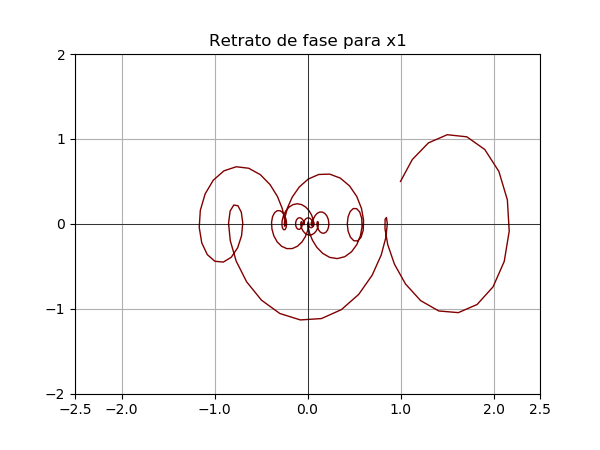
\includegraphics[width=.8\linewidth]{Ej2_41.png}
  \caption{Retrato de fase de $x_1$}
  \label{fig:sfig2}
\end{subfigure}
\begin{subfigure}{.55\textwidth}
  \centering
  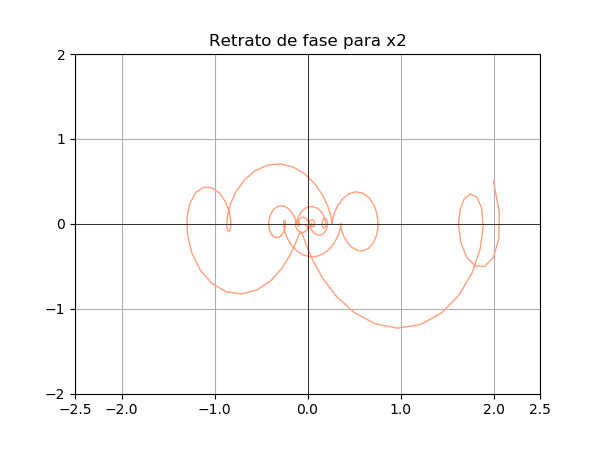
\includegraphics[width=.8\linewidth]{Ej2_42.png}
  \caption{Retrato de fase de $x_2$}
  \label{fig:sfig2}
\end{subfigure}
\begin{subfigure}{.55\textwidth}
  \centering
  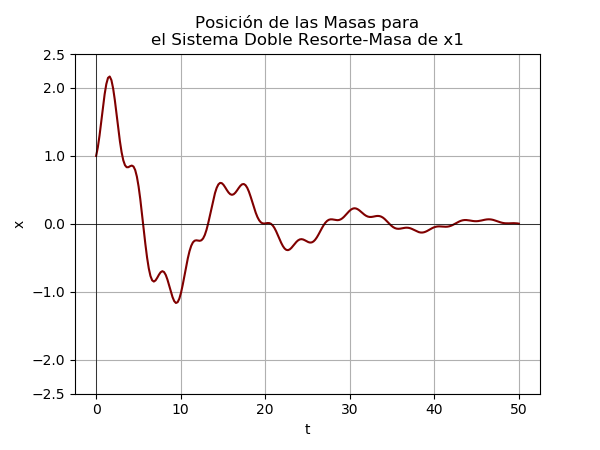
\includegraphics[width=.8\linewidth]{Ej2_43.png}
  \caption{Posición $x_1$ contra tiempo}
  \label{fig:sfig2}
\end{subfigure}
\begin{subfigure}{.55\textwidth}
  \centering
  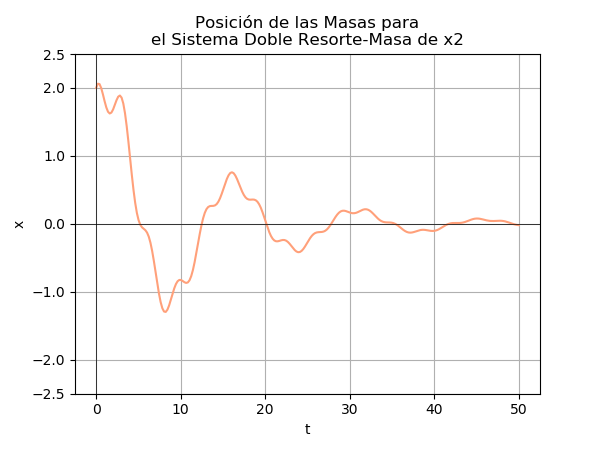
\includegraphics[width=.8\linewidth]{Ej2_44.png}
  \caption{Posición $x_2$ contra tiempo}
  \label{fig:sfig2}
\end{subfigure}
\begin{subfigure}{.55\textwidth}
  \centering
  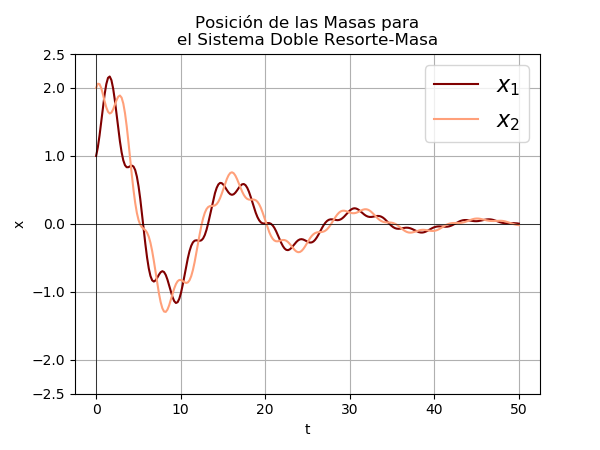
\includegraphics[width=.8\linewidth]{Ej2_45.png}
  \caption{Gráfica de $x_1$ y $x_2$}
  \label{fig:sfig2}
\end{subfigure}
\begin{subfigure}{.55\textwidth}
  \centering
  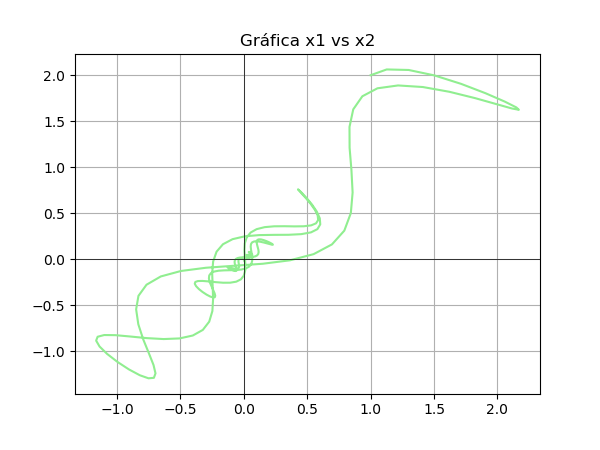
\includegraphics[width=.8\linewidth]{Ej2_46.png}
  \caption{Gráfica $x_1$ vs $x_2$}
  \label{fig:sfig2}
\end{subfigure}
\end{figure}

\subsection{Añadiendo no linealidad}
Para el caso en el que las fuerzas restauradoras de los resortes ya no obedezcan la Ley de Hooke, se debe modificar el modelo que se tenia. Ahora habrá una nueva constante, la cual será $\mu$ , en donde el modelo queda de la siguiente manera: \\

\centerline{$m_1 \ddot x_1 = -\delta \dot x_1 -k_1x_1 - k_2(x_1-x_2) + \mu_1 (x_1-x_2)^3$}
\centerline{$m_2 \ddot x_2 = -\delta \dot x_2 -k_2(x_2-x_1) + \mu_2 (x_2-x_1)^3$}
$    $

La solución para estas ecuaciones son mas complicadas y se comportan de una manera mas extraña que los modelos lineales. Y aunque usemos un método numérico este perderá exactitud conforme pasa el tiempo. A continuación se presentan algunos ejemplos. \\

\noindent \textit{3.1 Asume $m_1 = m_2 = 1$. Describe el movimiento para un sistema de resortes con $k_1=0.4$ y $k_2=1.808$, con coeficientes de amortiguamiento $\delta_1=0$ y $\delta_2=0$, coeficientes de no lineales de $\mu_1=-1/6$ y $\mu_2=-1/10$ con condiciones iniciales de $(x_1(0), \dot x_1(0), x_2(0), \dot x_2(0)$)=$(1,0,-1/2,0)$.}\\

Como no hay amortiguamiento las oscilaciones parecen ser casi periodicas, y al graficar $x_1$ con $x_2$ contra el tiempo, podemos observar como sus movimientos parecen estar fuera de fase. Podemos observar como debido a la no linealidad, el modelo es mas sensible a las condiciones iniciales. \\ \\

\begin{figure}[h!]
    \centering
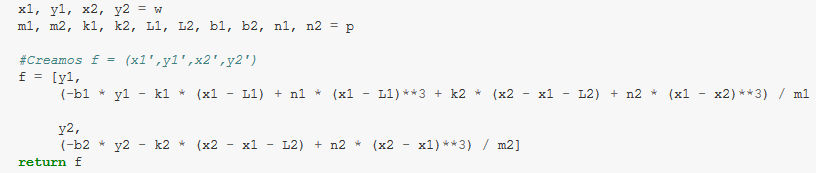
\includegraphics[width=5in]{Cod8.png}
\end{figure}

\begin{figure}[h!]
    \centering
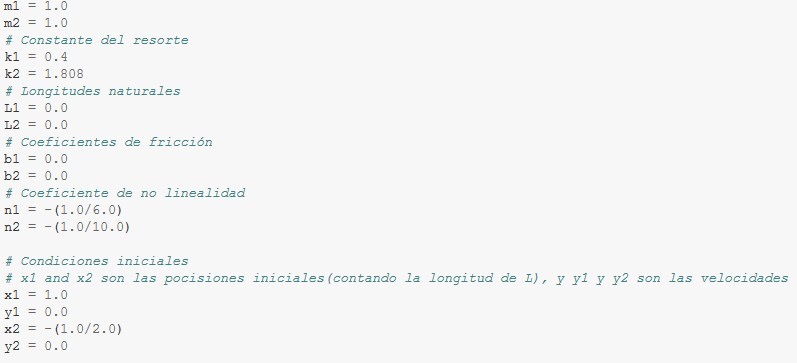
\includegraphics[width=5in]{Cod9.png}
\end{figure}

En el código solamente se edito la ecuación principal para añadir los nuevos coeficientes, dándoles los valores correspondientes. El resto se realizo de la misma manera que en los ejemplos anteriores. Las graficas resultantes fueron:

\begin{figure}[h!]
\begin{subfigure}{.55\textwidth}
  \centering
  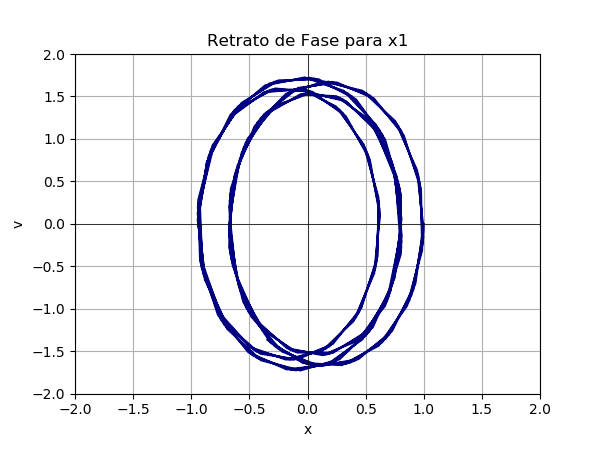
\includegraphics[width=.8\linewidth]{Ej3_11.png}
  \caption{Retrato de fase de $x_1$}
  \label{fig:sfig2}
\end{subfigure}
\begin{subfigure}{.55\textwidth}
  \centering
  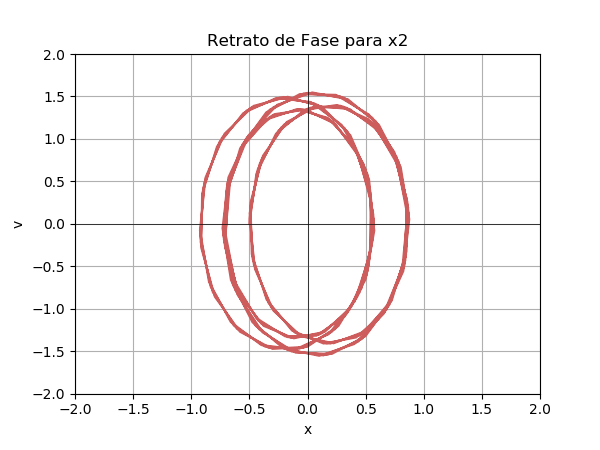
\includegraphics[width=.8\linewidth]{Ej3_12.png}
  \caption{Retrato de fase de $x_2$}
  \label{fig:sfig2}
\end{subfigure}
\begin{subfigure}{.55\textwidth}
  \centering
  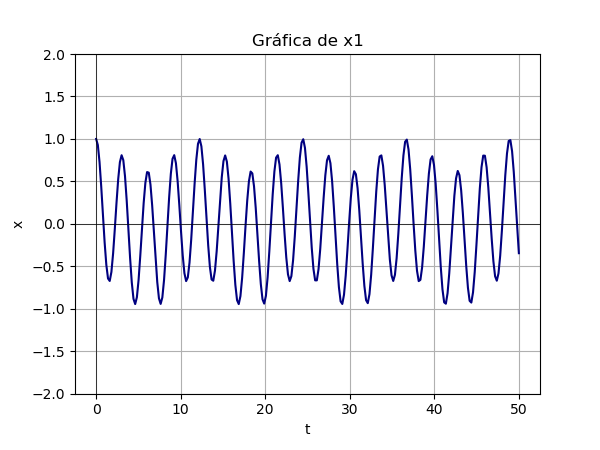
\includegraphics[width=.8\linewidth]{Ej3_13.png}
  \caption{Posición $x_1$ contra tiempo}
  \label{fig:sfig2}
\end{subfigure}
\begin{subfigure}{.55\textwidth}
  \centering
  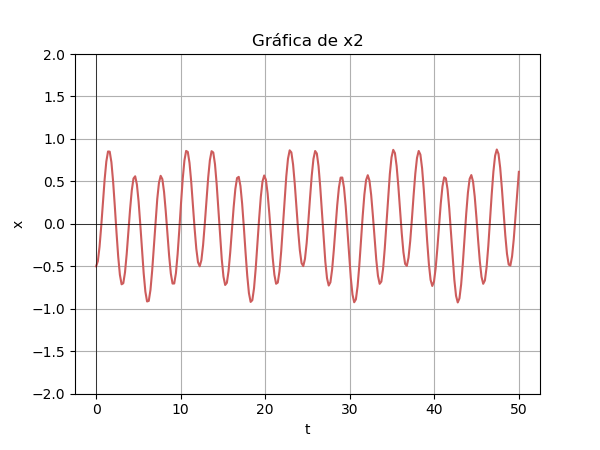
\includegraphics[width=.8\linewidth]{Ej3_14.png}
  \caption{Posición $x_2$ contra tiempo}
  \label{fig:sfig2}
\end{subfigure}
\begin{subfigure}{.55\textwidth}
  \centering
  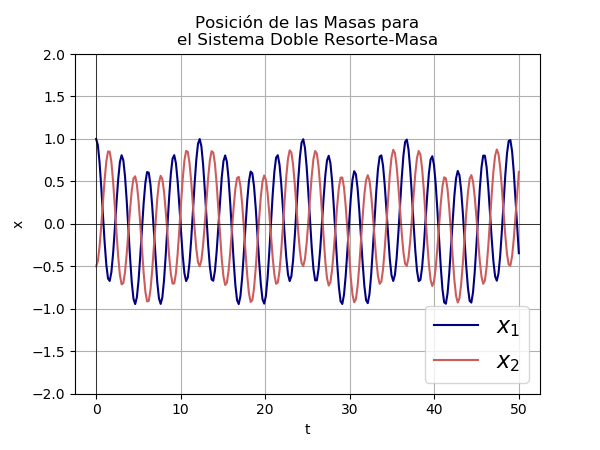
\includegraphics[width=.8\linewidth]{Ej3_15.png}
  \caption{Gráfica de $x_1$ y $x_2$}
  \label{fig:sfig2}
\end{subfigure}
\begin{subfigure}{.55\textwidth}
  \centering
  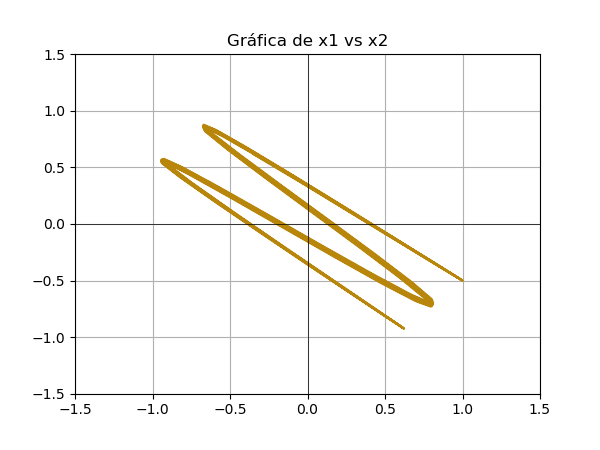
\includegraphics[width=.8\linewidth]{Ej3_16.png}
  \caption{Gráfica $x_1$ vs $x_2$}
  \label{fig:sfig2}
\end{subfigure}
\end{figure}

\pagebreak 

\noindent \textit{3.2 Asume $m_1 = m_2 = 1$. Describe el movimiento para un sistema de resortes con $k_1=0.4$ y $k_2=1.808$, con coeficientes de amortiguamiento $\delta_1=0$ y $\delta_2=0$, coeficientes de no lineales de $\mu_1=-1/6$ y $\mu_2=-1/10$ con condiciones iniciales de $(x_1(0), \dot x_1(0), x_2(0), \dot x_2(0)$)=$(-0.5,1/2,3.001,5.9)$.}\\

Este ejemplo tiene los mismos datos que el ejemplo anterior, solamente cambian las condiciones iniciales, en donde podemos observar, como un simple cambio hace que las graficas cambien bruscamente. 

\begin{figure}[h!]
\begin{subfigure}{.55\textwidth}
  \centering
  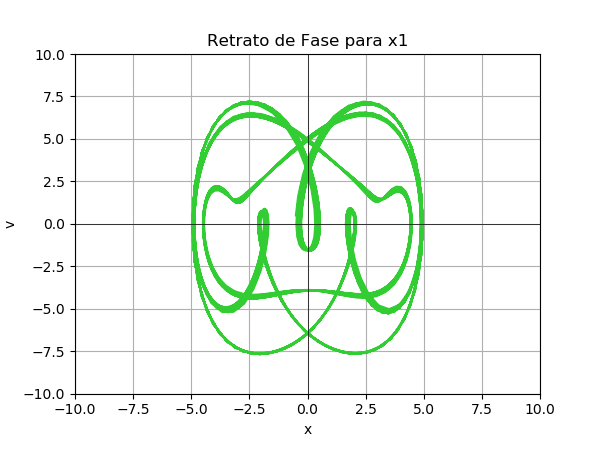
\includegraphics[width=.8\linewidth]{Ej3_21.png}
  \caption{Retrato de fase de $x_1$}
  \label{fig:sfig2}
\end{subfigure}
\begin{subfigure}{.55\textwidth}
  \centering
  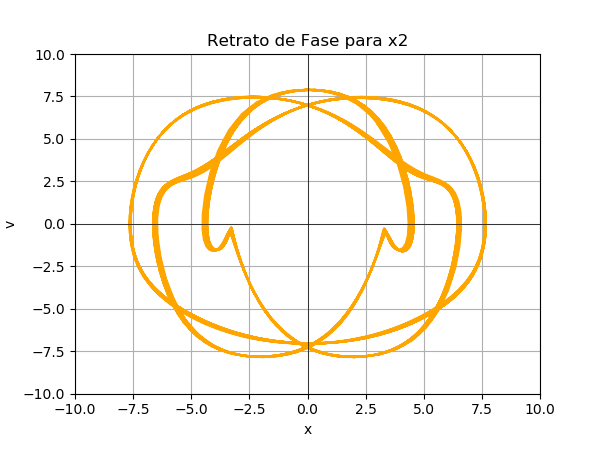
\includegraphics[width=.8\linewidth]{Ej3_22.png}
  \caption{Retrato de fase de $x_2$}
  \label{fig:sfig2}
\end{subfigure}
\end{figure}

\begin{figure}[h!]
    \centering
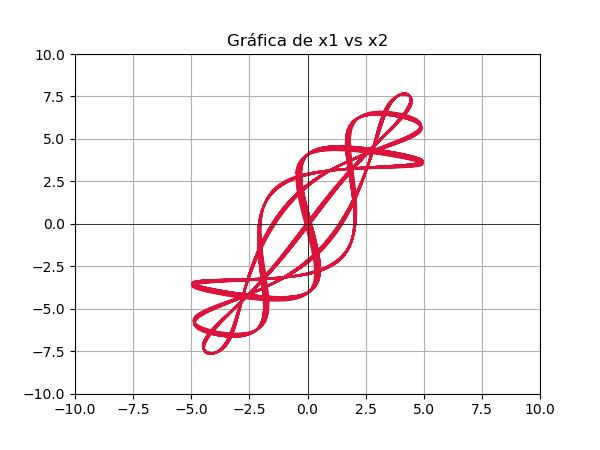
\includegraphics[width=5in]{Ej3_23.png}
\end{figure}

\pagebreak 

\noindent \textit{3.3 Asume $m_1 = m_2 = 1$. Describe el movimiento para un sistema de resortes con $k_1=0.4$ y $k_2=1.808$, con coeficientes de amortiguamiento $\delta_1=0$ y $\delta_2=0$, coeficientes de no lineales de $\mu_1=-1/6$ y $\mu_2=-1/10$ con condiciones iniciales de $(x_1(0), \dot x_1(0), x_2(0), \dot x_2(0)$)=$(-0.6,1/2,3.001,5.9)$.}\\

Este ejemplo tiene los mismos datos que el ejemplo anterior, pero ahora el unico cambio que existe es una diferencia de 0.1 en una de las posiciones iniciales, haciendo notar una vez mas que el mas simple cambio a las condiciones iniciales afectan mucho a los sistemas no lineales.

\begin{figure}[h!]
\begin{subfigure}{.55\textwidth}
  \centering
  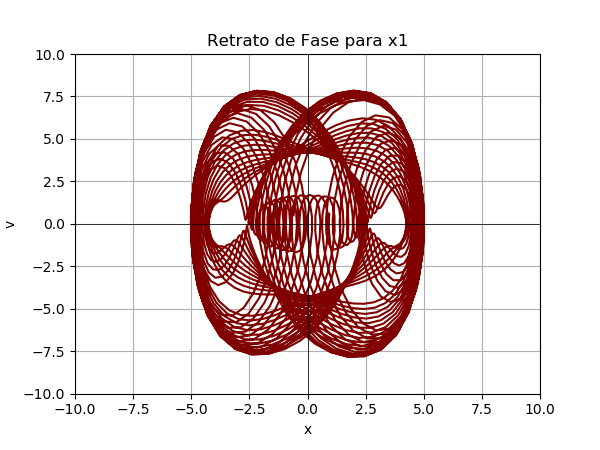
\includegraphics[width=.8\linewidth]{Ej3_31.png}
  \caption{Retrato de fase de $x_1$}
  \label{fig:sfig2}
\end{subfigure}
\begin{subfigure}{.55\textwidth}
  \centering
  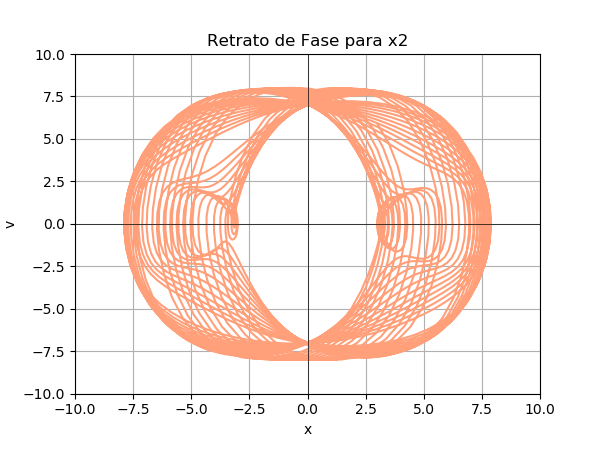
\includegraphics[width=.8\linewidth]{Ej3_32.png}
  \caption{Retrato de fase de $x_2$}
  \label{fig:sfig2}
\end{subfigure}
\end{figure}

\begin{figure}[h!]
    \centering
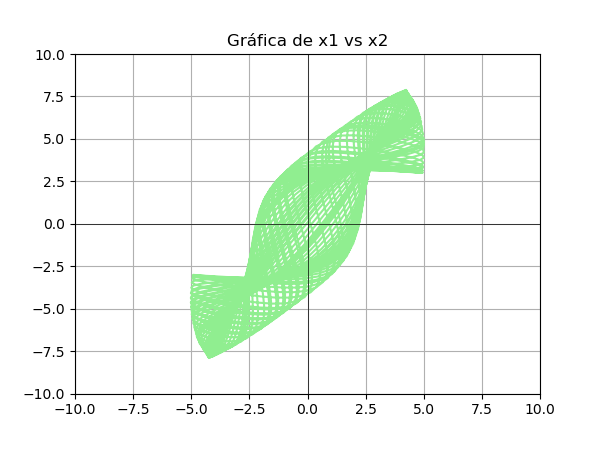
\includegraphics[width=5in]{Ej3_33.png}
\end{figure}

\pagebreak

\subsection{Añadiendo forzamiento}
Es muy fácil añadirle fuerza externa al modelo pasado, en donde incluso puede añadirsele una fuerza a cada masa simultáneamente, siendo o no iguales. Suponiendo una fuerza senoidal simple el modelo queda: \\

\centerline{$m_1 \ddot x_1 = -\delta \dot x_1 -k_1x_1 - k_2(x_1-x_2) + \mu_1 (x_1-x_2)^3 + F_1 cos(w_1t)$}
\centerline{$m_2 \ddot x_2 = -\delta \dot x_2 -k_2(x_2-x_1) + \mu_2 (x_2-x_1)^3 + F_2 cos(w_2t)$}
$    $

El rango de movimiento para este tipo de modelos tiene muchas posibilidades, resonancia no lineal, el periodo de solución comparte el mismo periodo con el del forzamiento (soluciones armónicas) e incluso soluciones subarmónicas.  Las condiciones para que esto pase son muy difíciles de especificar, por lo cual para cerrar, se presenta un ejemplo final: \\ 

\noindent \textit{4.1 Asume $m_1 = m_2 = 1$. Describe el movimiento para un sistema de resortes con $k_1=2/5$ y $k_2=1$, con coeficientes de amortiguamiento $\delta_1=1/10$ y $\delta_2=1/5$, coeficientes de no lineales de $\mu_1=1/6$ y $\mu_2=1/10$, fuerzas de amplitud de $F_1=1/3$ y $F_2=3/5$ y frecuencias de amplitud de $w_1=1$ y $w_2=3/5$ con condiciones iniciales de $(x_1(0), \dot x_1(0), x_2(0), \dot x_2(0)$)=$(0.7,0,0.1,0)$.}\\

Como ahora si existe un coeficiente de amortiguamiento, para valores pequeños de t habrá un movimiento muy variable, pero para t grande se hara constante. Esto se puede observar en las graficas de limite de ciclo. El código solamente cambio de igual manera que la sección anterior, solamente se agrego los nuevos coeficientes y se le asignaron sus nuevos valores: \\ \\

\begin{figure}[h!]
    \centering
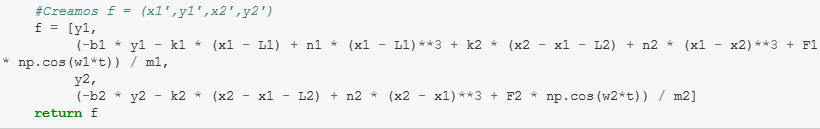
\includegraphics[width=6in]{Cod10.png}
\end{figure}

\begin{figure}[h!]
    \centering
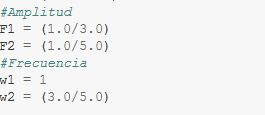
\includegraphics[width=4in]{Cod11.png}
\end{figure}

Las graficas obtenidas fueron: \\

\begin{figure}[h!]
\begin{subfigure}{.55\textwidth}
  \centering
  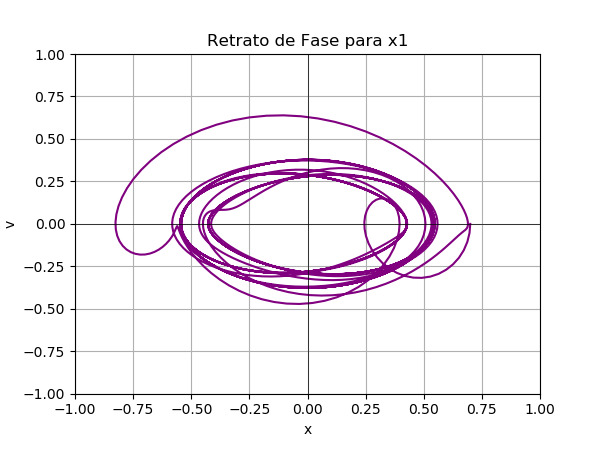
\includegraphics[width=.8\linewidth]{Ej4_11.png}
  \caption{Retrato de fase $x_1$}
  \label{fig:sfig2}
\end{subfigure}
\begin{subfigure}{.55\textwidth}
  \centering
  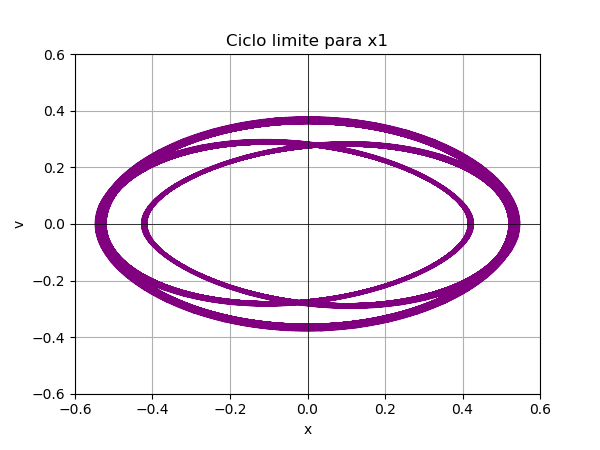
\includegraphics[width=.8\linewidth]{Ej4_15.png}
  \caption{Límite de ciclo para $x_1$}
  \label{fig:sfig2}
\end{subfigure}
\begin{subfigure}{.55\textwidth}
  \centering
  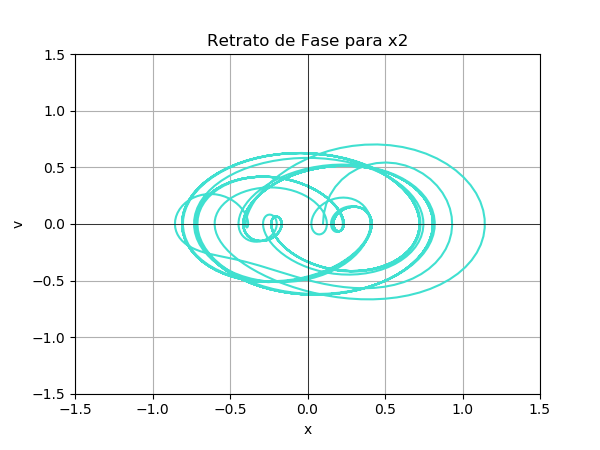
\includegraphics[width=.8\linewidth]{Ej4_12.png}
  \caption{Retrato de fase $x_2$}
  \label{fig:sfig2}
\end{subfigure}
\begin{subfigure}{.55\textwidth}
  \centering
  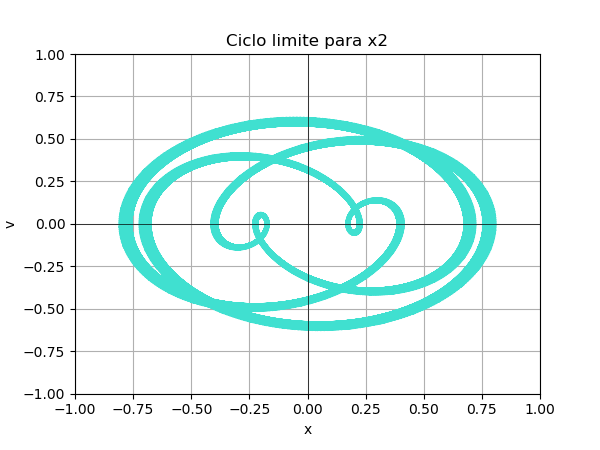
\includegraphics[width=.8\linewidth]{Ej4_16.png}
  \caption{Límite de ciclo para $x_2$}
  \label{fig:sfig2}
\end{subfigure}
\begin{subfigure}{.55\textwidth}
  \centering
  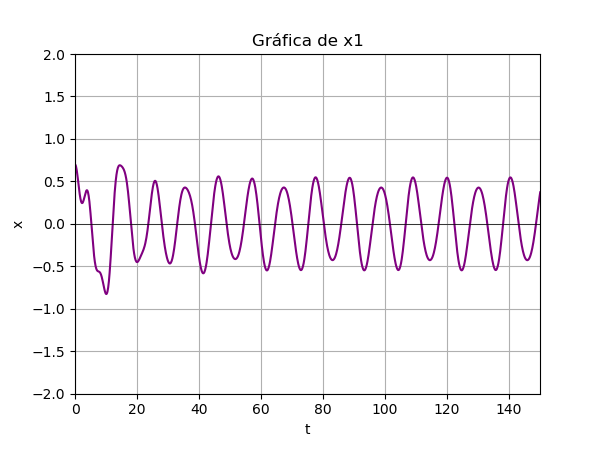
\includegraphics[width=.8\linewidth]{Ej4_13.png}
  \caption{Posición $x_1$ contra tiempo}
  \label{fig:sfig2}
\end{subfigure}
\begin{subfigure}{.55\textwidth}
  \centering
  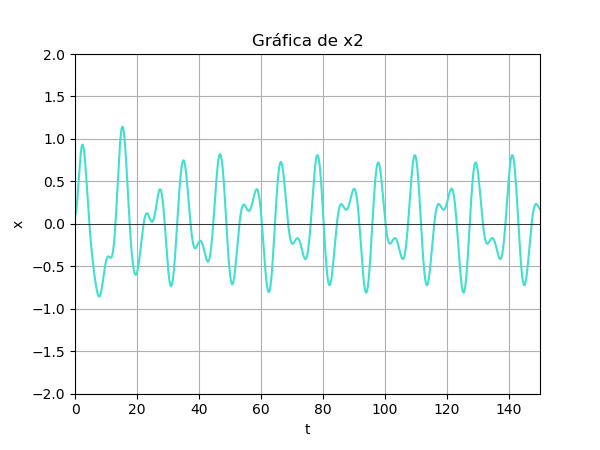
\includegraphics[width=.8\linewidth]{Ej4_14.png}
  \caption{Posición $x_1$ contra tiempo}
  \label{fig:sfig2}
\end{subfigure}
\end{figure}

\pagebreak

\section{Resultado analítico y resultado numérico}
Como en Python se realizo una aproximación numérica con los datos disponibles, y en el artículo se proporciona la solución analítica, es posible calcular el error relativo que hay entre nuestra aproximación y el valor real. Para hacer esto, en los primeros dos ejercicios, se imprimió en el archivo la definición del error relativo, restando el valor real al aproximado dividiendo esto entre el valor real. \\

Para el primer caso se obtuvo el error relativo calculando:

\begin{verbatim}
np.abs((w1[0]-(np.cos(np.sqrt(2.0)*t1)))/(np.cos(np.sqrt(2.0)*t1))) \\
np.abs((w1[2]-(2.0*np.cos(np.sqrt(2.0)*t1)))/(2.0*np.cos(np.sqrt(2)*t1)))
\end{verbatim}

En donde el primer comando es para $x_1$ y el segundo para $x_2$. Las graficas obtenidas del error relativo contra el tiempo, para el ejemplo 2.1 fueron:

\begin{figure}[h!]
\begin{subfigure}{.6\textwidth}
  \centering
  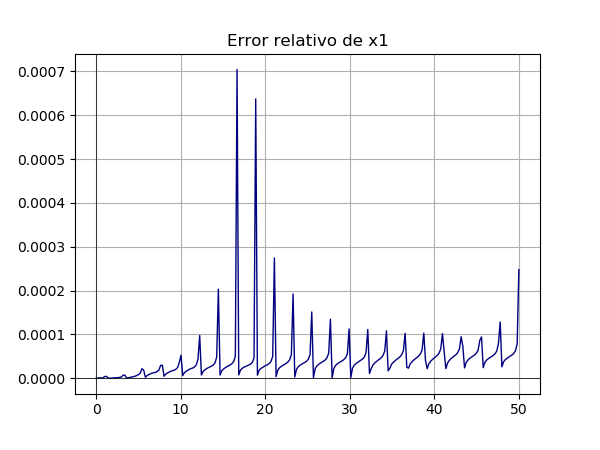
\includegraphics[width=.8\linewidth]{Ej2_14.png}
  \caption{Gráfica del error $x_1$ contra tiempo}
  \label{fig:sfig2}
\end{subfigure}
\begin{subfigure}{.6\textwidth}
  \centering
  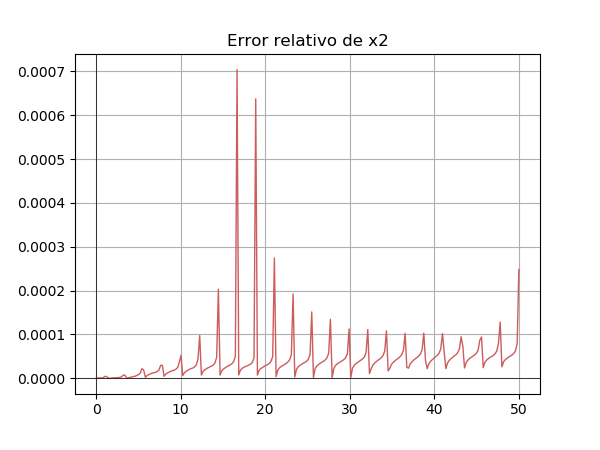
\includegraphics[width=.8\linewidth]{Ej2_15.png}
  \caption{Gráfica del error $x_2$ contra tiempo}
  \label{fig:sfig2}
\end{subfigure}
\end{figure}

Como se puede notar, los errores son muy pequeños, del orden de $7*10^{-3}$, y los errores entre $x_1$ y $x_2$ son idénticos. Este es el caso también para el ejemplo 2.2, donde el error es muy pequeño y casi igual para $x_1$ y $x_2$:

\begin{figure}[h!]
\begin{subfigure}{.6\textwidth}
  \centering
  \includegraphics[width=.6\linewidth]{Ej2_23.png}
  \caption{Gráfica del error $x_1$ contra tiempo}
  \label{fig:sfig2}
\end{subfigure}
\begin{subfigure}{.6\textwidth}
  \centering
  \includegraphics[width=.6\linewidth]{Ej2_24.png}
  \caption{Gráfica del error $x_2$ contra tiempo}
  \label{fig:sfig2}
\end{subfigure}
\end{figure}

\section{Conclusiones}
Ahora que se realizaron todos los ejemplos presentados por el articulo, podemos observar no solo lo interesante que es este tema de los resortes acoplados, si no también del poder que tiene Python para poder resolver problemas tan complicados como estos. \\

El mismo articulo menciona como incluso programas numericos no podrían tomar tan buenas aproximaciones de este tipo de modelos, pero Python logro reproducir todas las graficas en su totalidad. Esto solo pone en prueba lo poderoso que es Python y todas sus librería. 
\section{Bibliografía}
\begin{itemize}
    \item Temple H. Fay, Sarah Duncan Graham (2003) Coupled Spring Equations. Int. J. Educ. Math. Sci. Tech.. Vol. 34, No. 1, pp. 65-79. Recuperado de: http://math.oregonstate.edu/~gibsonn/Teaching/MTH323-010S15 \\ /Supplements/coupled\_spring.pdf
    \item Oscilaciones amortiguadas. (2010) Recuperado de:http://www.sc.ehu.es/sbweb/fisica/oscilaciones \\ /amortiguadas/amortiguadas.htm
\end{itemize}

Imagenes utilizadas:
\begin{itemize}
    \item http://srv2.fis.puc.cl/mediawiki/index.php/Osciladores\_Acoplados\_(Fiz0312)
\end{itemize}
\section{Apéndice}
\noindent\textbf {1. ¿Qué más te llama la atención de la actividad completa? ¿Que se te hizo menos interesante?} \\

Me gustaron mucho mas estos dos últimos temas que los pasados, ya que esto era algo totalmente nuevo. Este tema, como ya había mencionado anteriormente, es de mis favoritos de Mecánica II, y ver los modelos con sus respectivas soluciones fue muy divertido. \\

La verdad me gusto mucho esta práctica, no puedo decir que algo no me intereso. \\

\noindent\textbf {2. ¿De un sistema de masas acopladas como se trabaja en esta actividad, hubieras pensado que abre toda una nueva área de fenómenos no lineales? }\\

La verdad no. Cuando veiamos los casos "bien comportados" en cursos anteriores, nunca pense en los otros modelos que se podían presentar. Estos son mucho mas complicados y el hecho de poder estudiarlos numericamente con la ayuda de la programación es algo que me parece muy bien. \\ \\

\noindent\textbf {3. ¿Qué propondrías para mejorar esta actividad? ¿Te ha parecido interesante este reto?  } \\

Es muy interesante esta practica, y la verdad me pareció muy completa, sobre todo en la manera con la que se dividió. Me gustaría que hubiera mas referencias para poder entender mejor estos últimos dos temas, ya que el articulo casi no menciona mucho de ellos. \\

\noindent\textbf {4. ¿Quisieras estudiar mas este tipo de fenómenos no lineales?} \\

Si, es algo muy interesante.
\end{document}